\documentclass[10pt]{beamer}

% packages
\usepackage[utf8]{inputenc}

\usepackage{multirow,rotating}
\usepackage{color}
\usepackage{hyperref}
\usepackage{tikz-cd}
\usepackage{array}
\usepackage{siunitx}
\usepackage{mathtools,nccmath}%
\usepackage{etoolbox, xparse} 
\usetheme{CambridgeUS}
\usepackage{graphicx}
\usecolortheme{dolphin}
\usepackage{listings}
\usepackage{bibentry}
\usepackage{natbib}

% layout setup
%% Memoir layout setup

%% NOTE: You are strongly advised not to change any of them unless you
%% know what you are doing.  These settings strongly interact in the
%% final look of the document.

% Dependencies
\usepackage{USIlogo}

% Turn extra space before chapter headings off.
\setlength{\beforechapskip}{0pt}

\nonzeroparskip
\parindent=0pt
\defaultlists

% Chapter style redefinition
\makeatletter

\if@twoside
  \pagestyle{Ruled}
  \copypagestyle{chapter}{Ruled}
\else
  \pagestyle{ruled}
  \copypagestyle{chapter}{ruled}
\fi
\makeoddhead{chapter}{}{}{}
\makeevenhead{chapter}{}{}{}
\makeheadrule{chapter}{\textwidth}{0pt}
\copypagestyle{abstract}{empty}

\makechapterstyle{bianchimod}{%
  \chapterstyle{default}
  \renewcommand*{\chapnamefont}{\normalfont\Large\sffamily}
  \renewcommand*{\chapnumfont}{\normalfont\Large\sffamily}
  \renewcommand*{\printchaptername}{%
    \chapnamefont\centering\@chapapp}
  \renewcommand*{\printchapternum}{\chapnumfont {\thechapter}}
  \renewcommand*{\chaptitlefont}{\normalfont\huge\sffamily}
  \renewcommand*{\printchaptertitle}[1]{%
    \hrule\vskip\onelineskip \centering \chaptitlefont\textbf{\vphantom{gyM}##1}\par}
  \renewcommand*{\afterchaptertitle}{\vskip\onelineskip \hrule\vskip
    \afterchapskip}
  \renewcommand*{\printchapternonum}{%
    \vphantom{\chapnumfont {9}}\afterchapternum}}

% Use the newly defined style
\chapterstyle{bianchimod}

\setsecheadstyle{\Large\bfseries\sffamily}
\setsubsecheadstyle{\large\bfseries\sffamily}
\setsubsubsecheadstyle{\bfseries\sffamily}
\setparaheadstyle{\normalsize\bfseries\sffamily}
\setsubparaheadstyle{\normalsize\itshape\sffamily}
\setsubparaindent{0pt}

% Set captions to a more separated style for clearness
\captionnamefont{\sffamily\bfseries\footnotesize}
\captiontitlefont{\sffamily\footnotesize}
\setlength{\intextsep}{16pt}
\setlength{\belowcaptionskip}{1pt}

% Set section and TOC numbering depth to subsection
\setsecnumdepth{subsection}
\settocdepth{subsection}

%% Titlepage adjustments
\pretitle{\vspace{0pt plus 0.7fill}\begin{center}\HUGE\sffamily\bfseries}
\posttitle{\end{center}\par}
\preauthor{\par\begin{center}\let\and\\\Large\sffamily}
\postauthor{\end{center}}
\predate{\par\begin{center}\Large\sffamily}
\postdate{\end{center}}

\def\@advisors{}
\newcommand{\advisors}[1]{\def\@advisors{#1}}
\def\@coadvisors{}
\newcommand{\coadvisors}[1]{\def\@coadvisors{#1}}
\def\@department{}
\newcommand{\department}[1]{\def\@department{#1}}
\def\@thesistype{}
\newcommand{\thesistype}[1]{\def\@thesistype{#1}}

\renewcommand{\maketitlehooka}{\noindent\USIlogo[2in]}

\renewcommand{\maketitlehookb}{\vspace{1in}%
  \par\begin{center}\Large\sffamily\@thesistype\end{center}}

\renewcommand{\maketitlehookd}{%
  \vfill\par
  \begin{flushright}
    \sffamily
    \@advisors\par
    \@coadvisors\par
    \@department, USI Lugano
  \end{flushright}
}

\checkandfixthelayout

\setlength{\droptitle}{-48pt}

\makeatother

% This defines how theorems should look. Best leave as is.
\theoremstyle{plain}
\setlength\theorempostskipamount{0pt}

%%% Local Variables:
%%% mode: latex
%%% TeX-master: "thesis"
%%% End:


%------------------------------------------------------------

\titlegraphic{%

\includegraphics[width=3.0cm]{ua_seal.png}
}

\title[USI]{Energy Market Analysis Using Kernel Methods}%title
%\subtitle{ }%%subtitle
\author[Luca Pernigo]{L. Pernigo}%%authors

\institute[USI]{Università della Svizzera italiana\inst{1}}
\date[\textcolor{white}{Energy Market Analysis KernelMethods, 2024}]
{Advisor: Prof.\ Dr.\ M.\ Multerer\\
Co-Advisor: Dr.\ D.\ Baroli\\
June 17, 2024}

% ------Contents below------
%------------------------------------------------------------

\begin{document}

%The next statement creates the title page.
\frame{\titlepage}
\begin{frame}
\frametitle{Outline}
\tableofcontents
\end{frame}


%------------------------------------------------------------
% motivation
% ch 1,2
% motivation
% ch 1,2
\section{Motivation}

\begin{frame}{Motivation}
    aaa
\end{frame}




\begin{frame}{Objectives}
    
\end{frame}

% energy market
% ch 5
% Chapter explaining the energy market
% Chapter 9 of https://pubs.naruc.org/pub.cfm?id=536E10A7-2354-D714-5191-A8AAFE45D626

This chapter has two intents. Firstly, it summarizes several concepts for the newcomers to the field of electricity markets. Secondly, it discusses trends and challenges undergoing in the power sector. Such developments motivate the need for robust and efficient forecasting techniques in the context of electricity markets.


\section{Electricity distribution network}
Electricity is generated by power plants which transfer it over the so called transmission level. Then, through the transmission network, this energy is transported at a high voltage over long distances. Finally, the voltage is reduced and the energy is moved into the distribution network. In a nutshell, transmision lines carry electric power from stations to substations while distribution lines carry electricity from substations to load points such as businesses, industries and homes, see figure \ref{electricity_network}.

\begin{figure}[!h]
    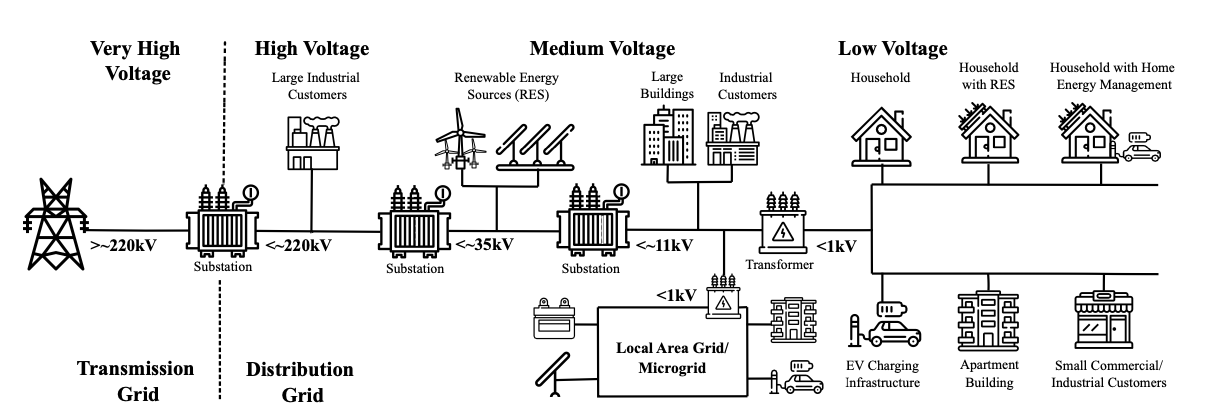
\includegraphics[width=\textwidth]{images/electricity_network.png}
    \caption{Electricity grid \cite{haben2021review}}
    \label{electricity_network}
\end{figure}


\section{Electricity markets}
Electricity markets have gone rapid changes all over the world during the last three decades.
Before this revolution, the power sector was a natural monopoly. In particular, it was characterized by a high vertical integration and by very little market competition. Better technologies in both transmission, generation and distribution are the reasons for such liberal shift. The rationale is simple, a competitive market promotes efficiency and stimulates technical innovation more than a monopoly does.
\\
During the nineties various wholesale electricity markets were established; for example in Chile, Great Britain, the scandinivian block, Australia, New Zealand, the US and Canada. Consequently, new participants, each with a specific task, entered the power market scenario.
\begin{itemize}
    \item Electricity generators produce electricity to be consumed.
    \item Electricity transmission owners 
    move high voltage electricity to electric utility companies whilst ensuring safe and reliable supply.
    \item Electricity grid operators are responsible for scheduling electricity over the transmission network in order to ensure supply demand balance.
    \item Electric utilities deliver power over local lines to consumers. 
    \item Retail energy suppliers purchase electricity in the wholesale market from electricity generators and resell it to consumers.
\end{itemize}
Notice, these functions are not mutually exclusive; that is an entity can provide one or more of these services.


\subsection{The marketplace}
We can differentiate between two kinds of electricity markets: power pools and power exchanges. In power pools, generators bid the prices at which they are willing to produce at different volumes. Then, the market clearing price (MCP) is determined by intersecting the aggregated supply curve and the estimated demand, left panel figure \ref{fig:pool_vs_echange}. Power pools are created on public initiatives of governments. Conversely, power exchanges are created through private agreements between generators, distributors and traders. This is the model followed by most of european countries.
The MCP in power exchanges is determined by the intersection of the aggregate supply curve and the aggregate demand curve, right panel figure \ref{fig:pool_vs_echange}.
\\
It is worth to mention the two biggest power exchanges: Epex and NordPool. Epex operates throughout continental europe. NordPool covers the nordinc and baltic contries.
\\
Moreover, we can differentiate between two popular types of auctions: uniform-price/marginal and pay as bid/discriminatory. Within the uniform price setting, suppliers offering less than the clearing price are paid that price. Analogously, consumers bidding more than the clearing price pay that price. On the other hand, in pay as bid auctions, suppliers are paid the exact price they bid for.


\begin{figure}[!h]
    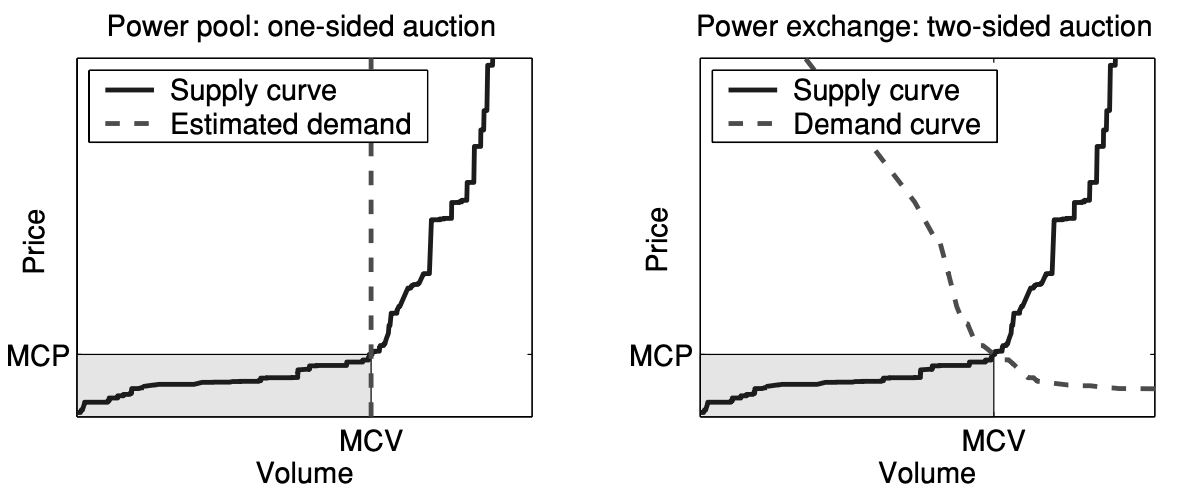
\includegraphics[width=\textwidth]{images/pool_vs_echange.png}
    \caption{Pool market versus power echange \cite{weron2006modeling}}
    \label{fig:pool_vs_echange}
\end{figure}

\subsection{How auctions work}
We can drill down on the auction types, the two most popular forms are day ahead and intraday auctions.
% https://medium.com/@brandonvar/day-ahead-and-intraday-electricity-markets-1eb121dcab47

% \subsection{Day ahead}
The day ahead market is based on a blind auction taking place every day of the year.
During these auctions, the prices of all hours for the next day are traded.
Market participants can enter their buy and sell orders until order book closure, which takes place at 12.00 PM. After that, the market establishes hourly prices by intersecting the demand and supply curves for each hour of the following day.

% \subsection{Intraday}
The intraday market consists of continous trading 24/7. A trade is executed as soon as a buy and a sell order mathch. Electricity can be traded an hour, half-hour, quarter or also 5 minutes before delivery. This enables market participants to balance their positions in real time, should they need to do so.

\subsection{Price peaks}
Electricity market are characterized by spikes in their spot prices; when this happens, the system price jumps abruptly and then drops back within a very short period.
This spikness follows from the non storability of electricity; that is, electricity has to be consumed as it is produced. Therefore, extreme load fluctuations combined with generation outages or transmission failures can result in price spikes.

% outages=interruzione
\subsection{Negative prices}
It is not unusual to observe negative prices in electricity markets, even though they are rare.
The causes of negative prices are inflexible power generation plants and low demand. With inflexibility, it is mean the fact that power sources cannot be switched off and restarted quickly and efficiently.
Thus, producers are faced with the decision of either stopping and restarting their power plant or selling their energy for a negative price; that is they pay consumers for consuming their energy.

\subsection{Nodal and zonal pricing}
Grid configuration and physical limits on electricity lines may lead to congestion. Local marginal price (LMP) and zonal market clearing pricing (ZMCP) are two types of pricing schemes utilized to handle it. The former is adopted in EU contries while the latter is used in the US, figure \ref{fig:eu_zonal} and figure \ref{fig:us_local}.
With zonal market clearing pricing, prices may differ between zones but are the same within the same area.
On the other hand, local marginal price is made up by summing the transmission congestion cost, generation marginal cost and the cost of marginal losses at different buses; buses is where a electicity line or several lines are connected.
\begin{figure}[!h]
    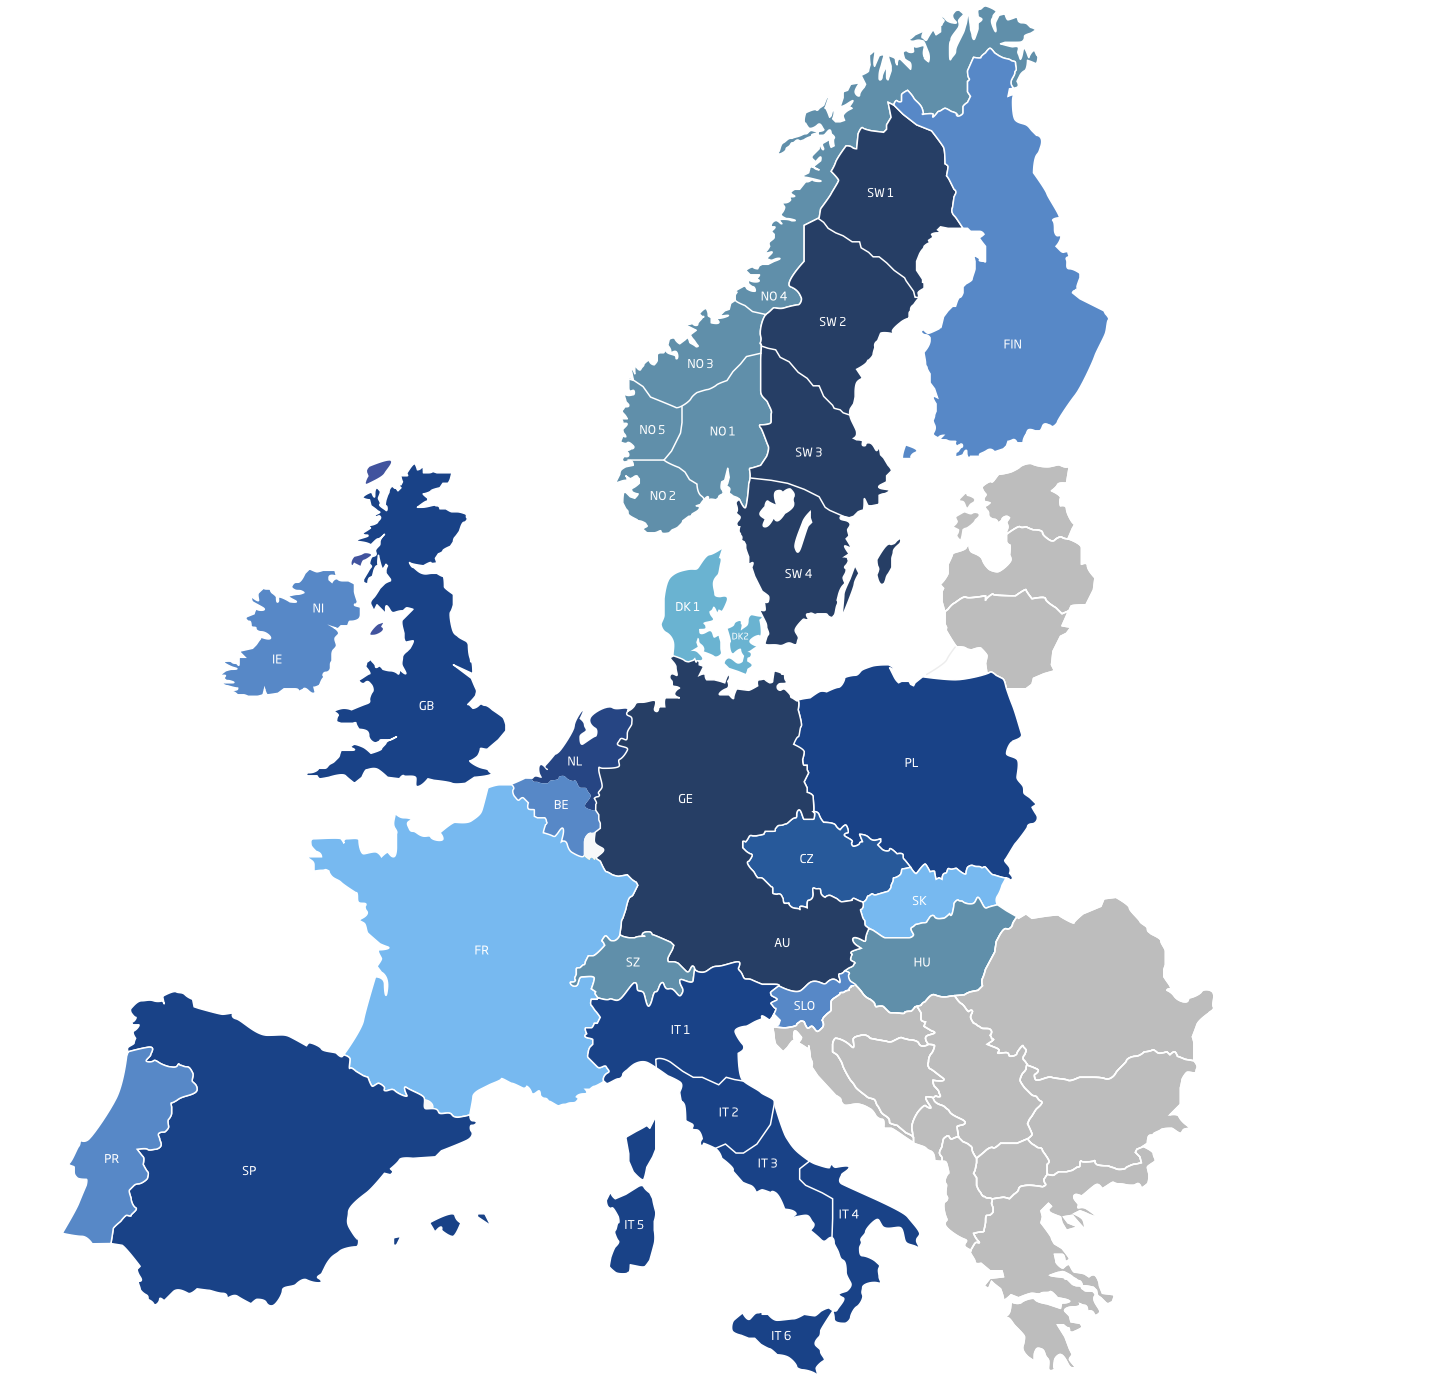
\includegraphics[width=\textwidth]{images/eu_zonal.png}
    \caption{Zonal pricing EU \cite{eu_zonal}}
    \label{fig:eu_zonal}
\end{figure}

\begin{figure}[!h]
    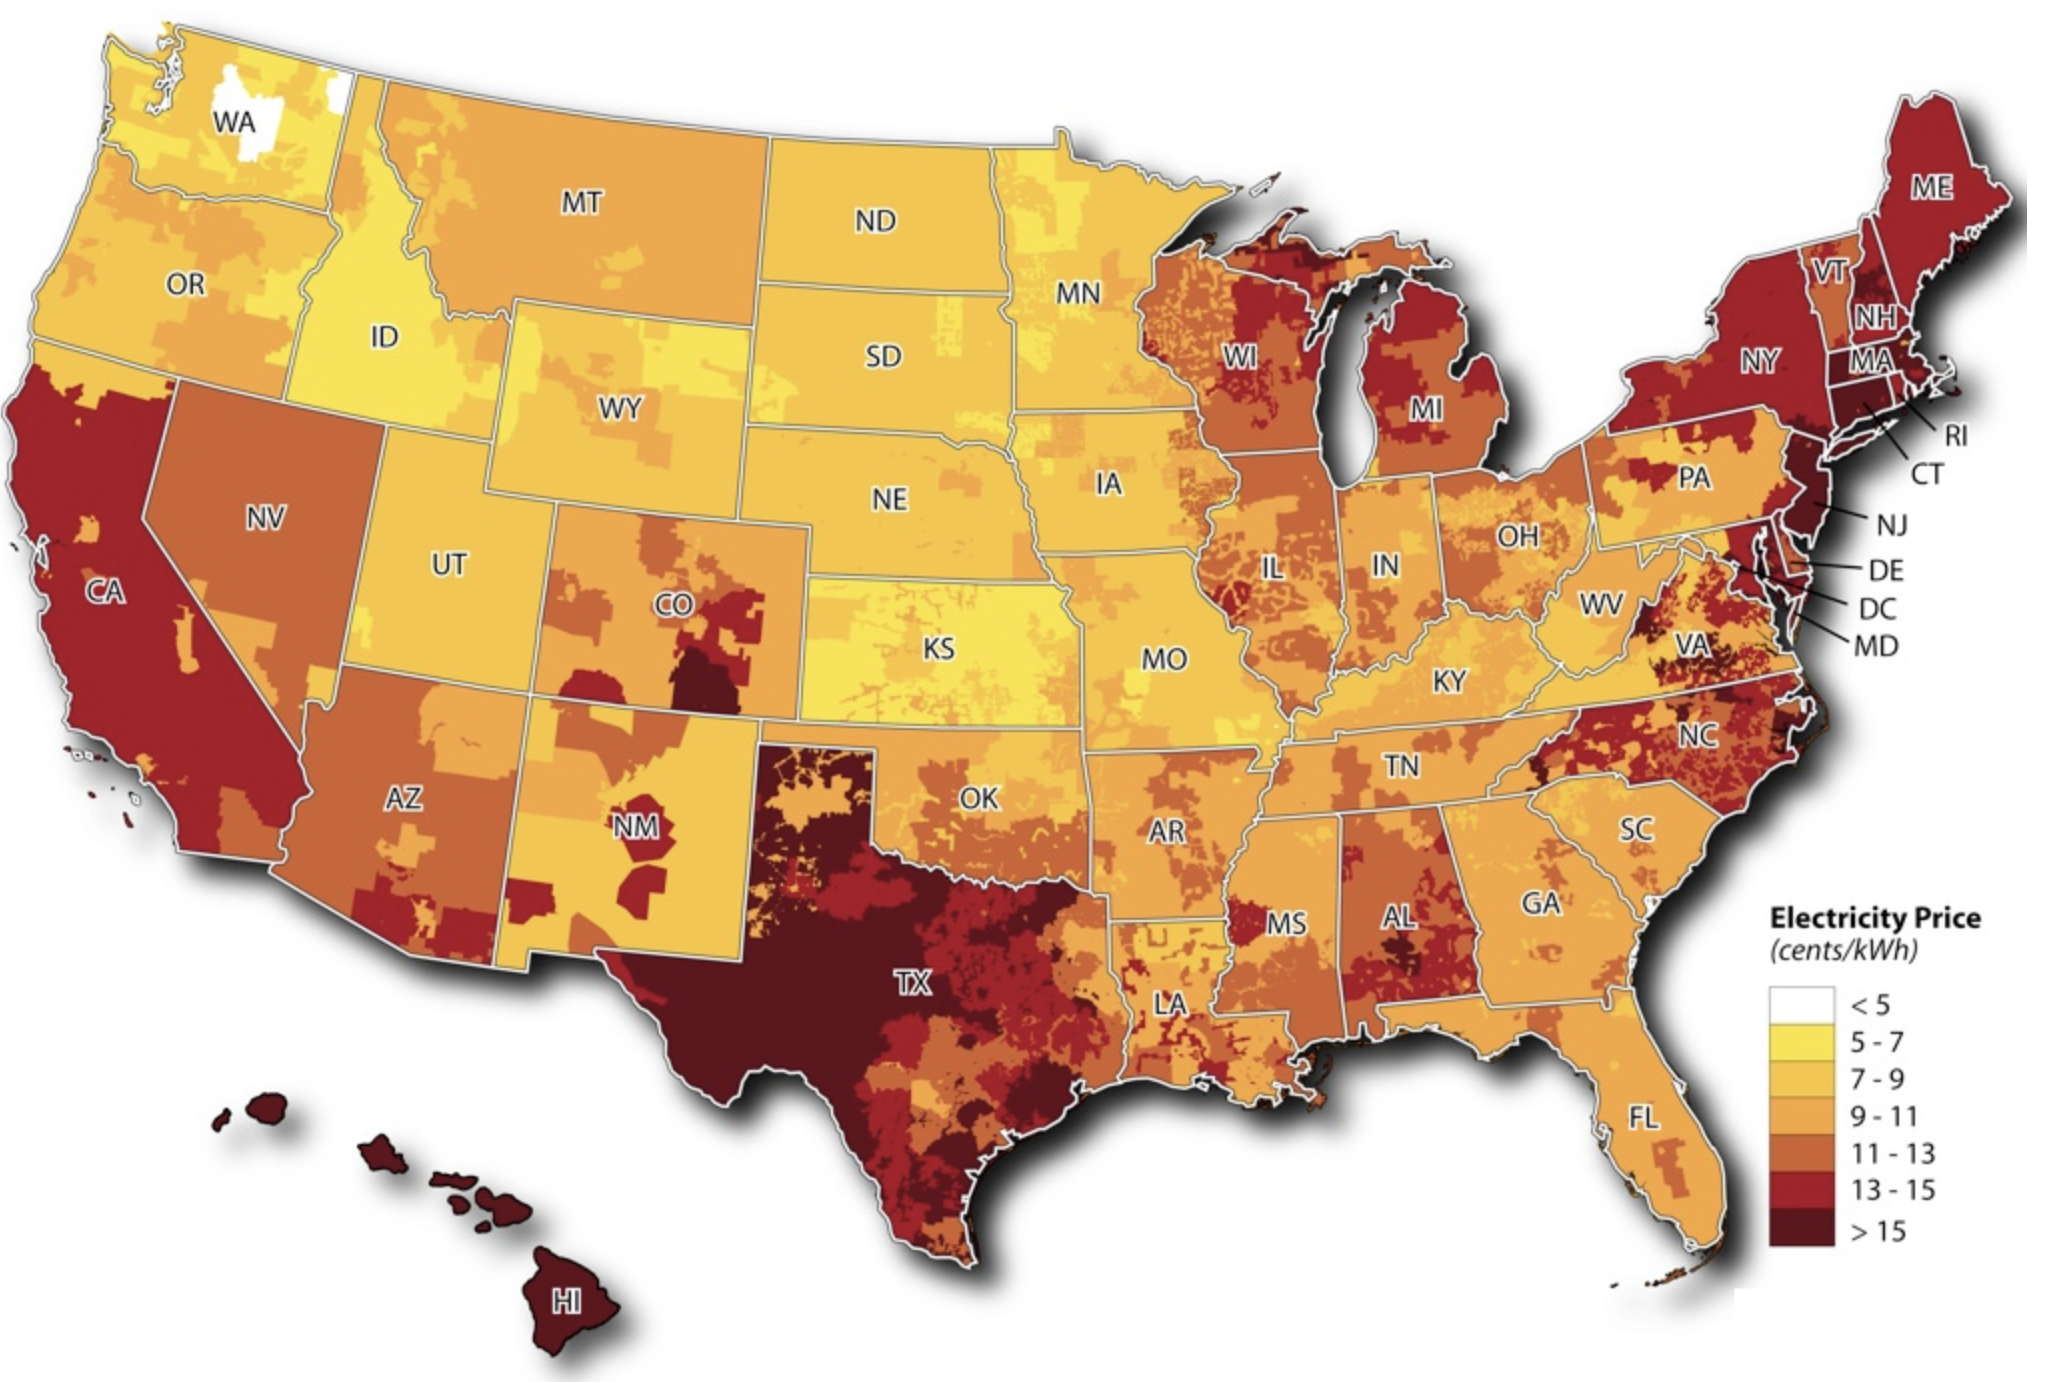
\includegraphics[width=\textwidth]{images/us_local.png}
    \caption{Local pricing US \cite{us_local}}
    \label{fig:us_local}
\end{figure}

% pensodino \subsection{Nodal and Zonal Pricing}
\section{Smart grids}
A smart meter is a digital device recording energy consumption in real time and communicating this data to the supplier and the consumer.
Deployment of smart grids and the digitalisation of the electricity network are intended to increase the energy efficiency of our networks.
The reason is that, smart metering and the electricity network digitalisation  will enable system operators to better monitor the network, plan their investments and manage infrastructure. 
All of this motivates for the need of efficient and robust tools to analyze the vast data resulting from the digitalisation of the power sector.

\section{Renewables}
% https://www.pnnl.gov/explainer-articles/renewable-integration
A pressing challenge facing policymakers today is the energy transition towards cleaner energy, see figure \ref{fig:electricity_production_by_source} for an up to date breakdown on energy production by source. Such move is intended to mitigate the effects of climate change and reduce pollution at the same time.
This transition passes through renewables integration into the electric grid. 
Nevertheless, integrating renewables into the existing electric grid involves several technical challenges. First, we need to develop infrastructures and technologies capable of connecting renewable power plants with the existing grid. For example, connecting renewables power plants located in remote and offshore locations to high voltage powerlines is not trivial.
Additionally, renewables such as wind and solar are characterized by seasonalities and depend heavily on weather conditions. Therefore, balancing the electricity network and mantaining stability will become harder for grid operators; they will need more flexibility in the grid and develop new approaches in order to achieve their goals.

\begin{figure}[!h]
    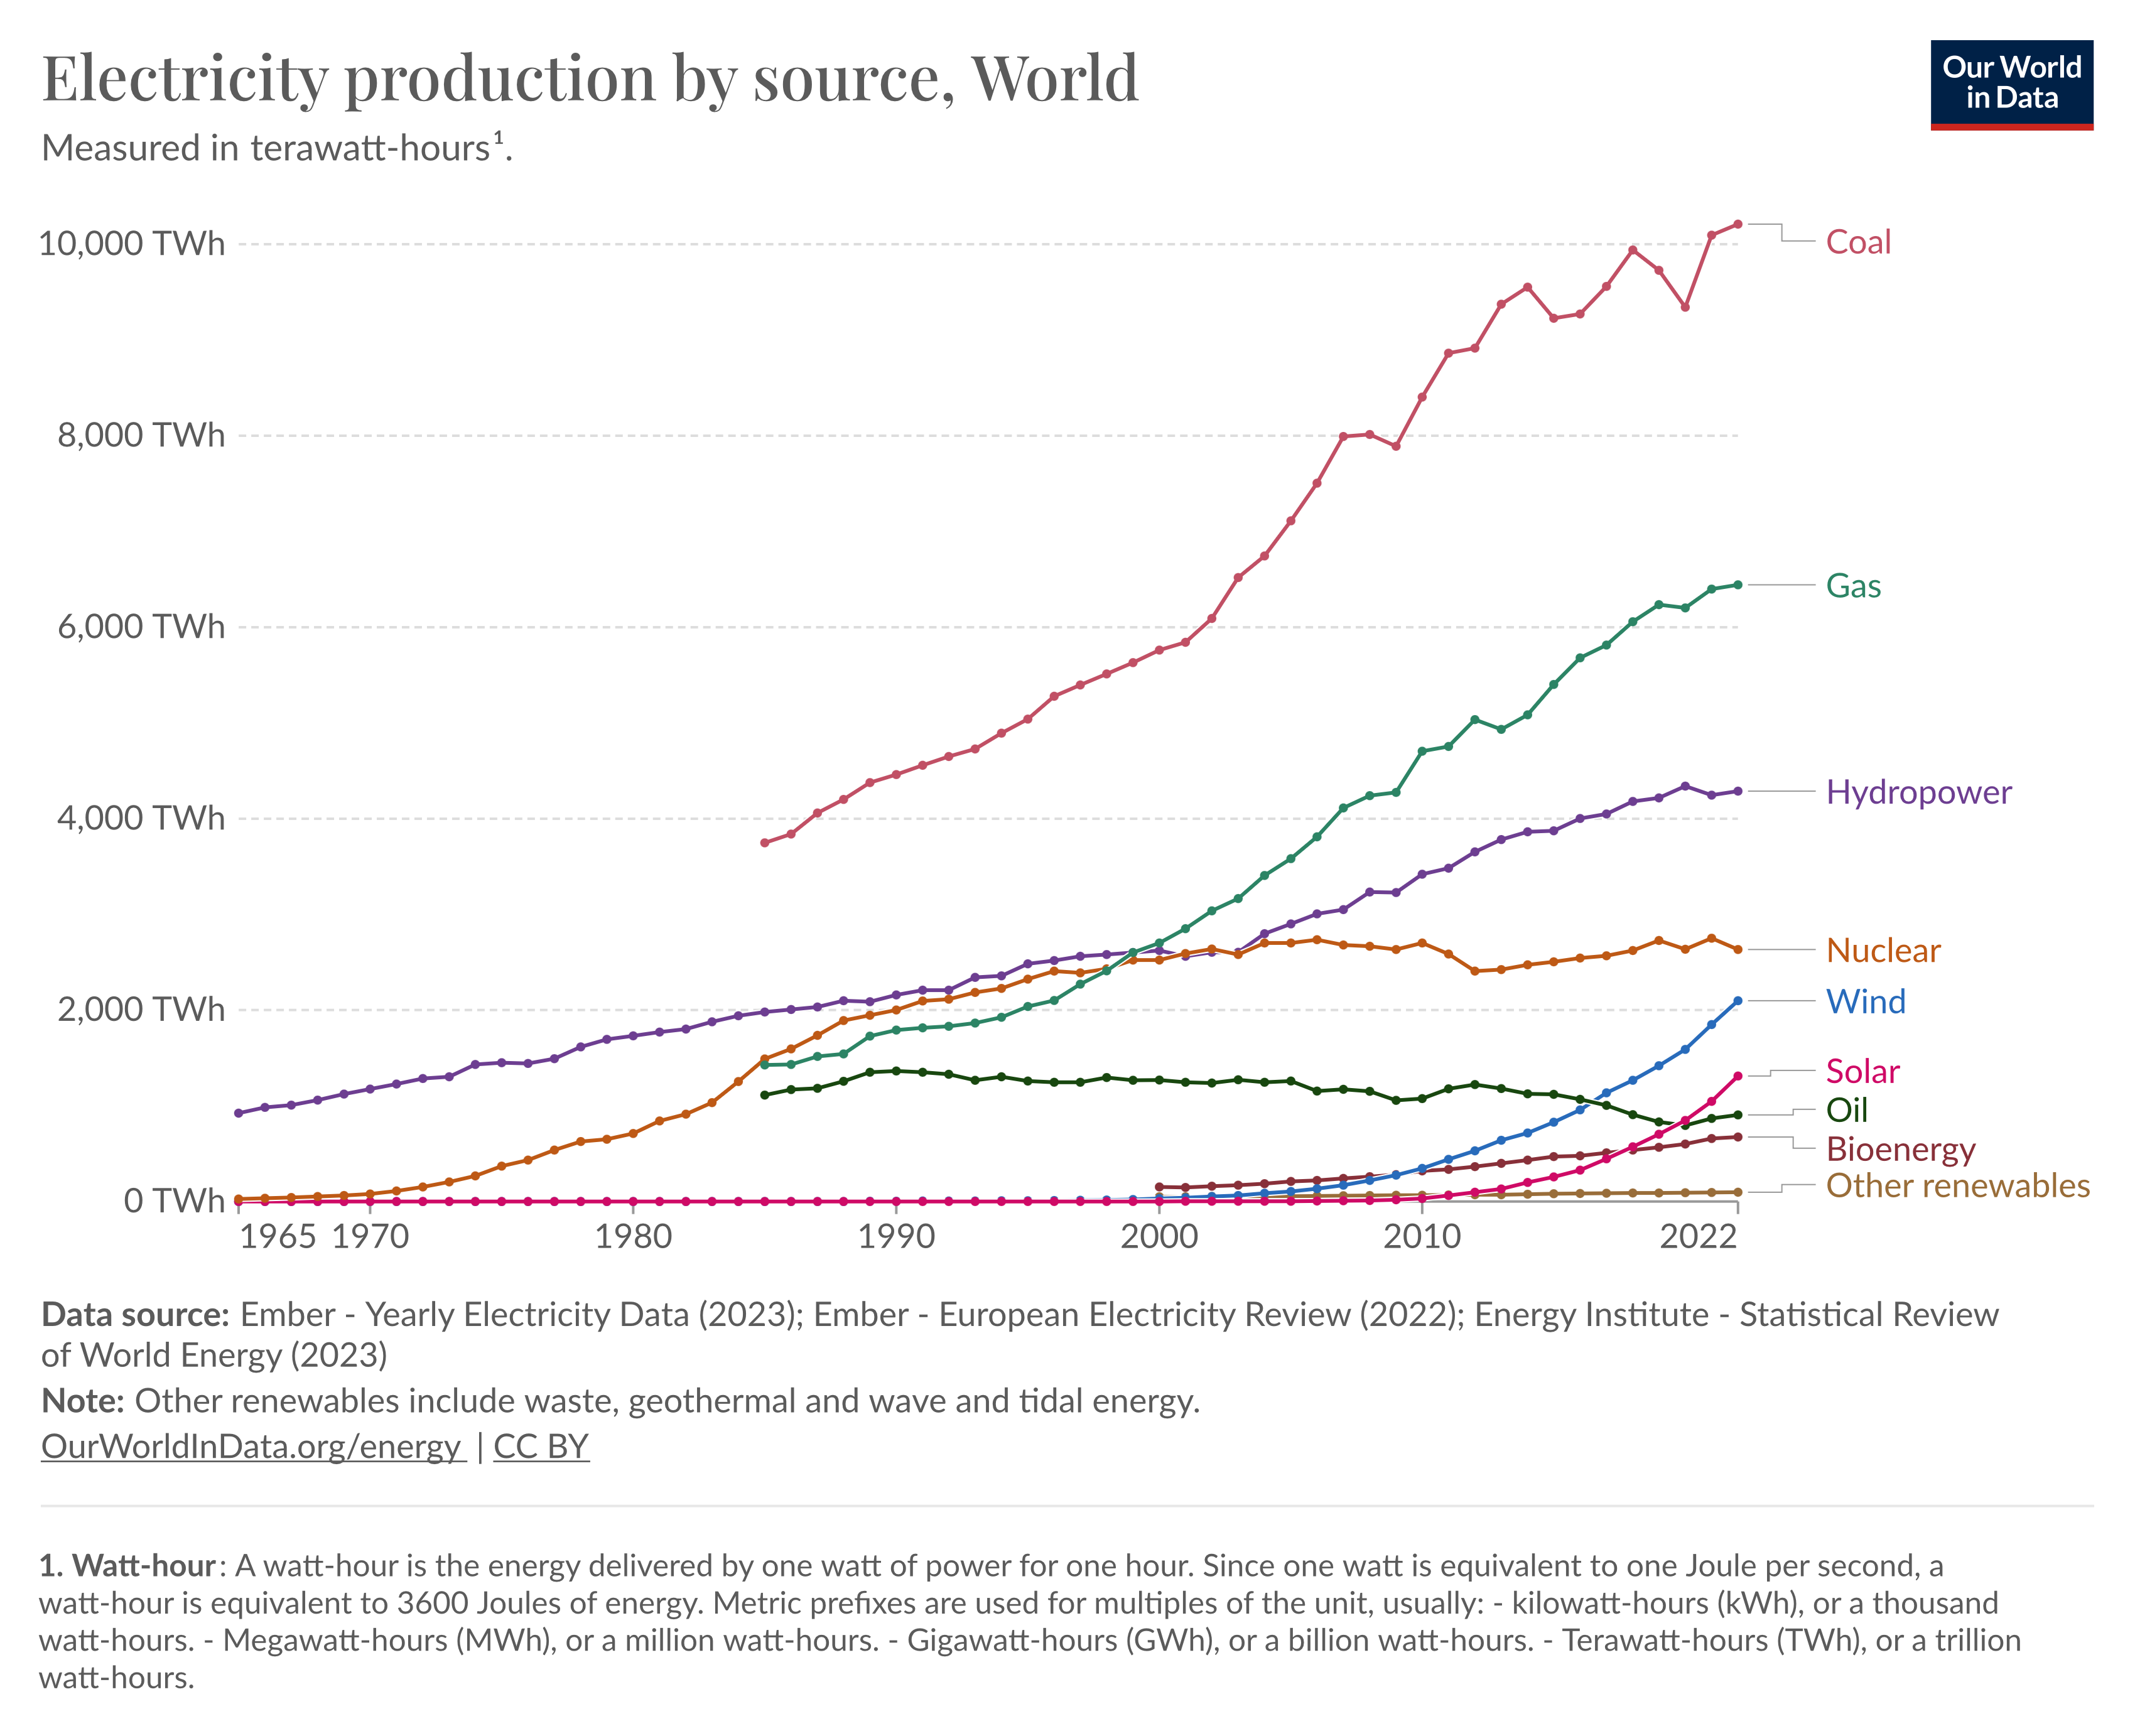
\includegraphics[width=\textwidth]{images/electricity-production-by-source.png}
    \caption{Electricity production by source}    
    \label{fig:electricity_production_by_source}
\end{figure}



% ef research
% ch 2, 4, 5
% ef research
% ch 2, 4, 5

\section{Energy forecasting research}


\subsection{Probabilistic scores}
\begin{frame}{Pinball loss}
    The pinball score or quantile score is used to measure the accuracy of a quantile forecast.
\begin{definition}
    The pinball loss is defined as
    $$
    \mathrm{Pinball}(y_{t},\hat{y}_{t,q},q)=
\begin{cases}
(q-1)(\hat{y}_{t,q}-y_{t}) & y_t > \hat{y}_{t,q} \\
q(\hat{y}_{t,q}-y_t) & y_t \leq \hat{y}_{t,q}
\end{cases}
$$
\end{definition}
\end{frame}


\begin{frame}{Pinball loss}
    The pinball loss is an asymmetric function, it weights its score differently depending on the error sign and on the quantile considered.
By averaging all the pinball losses over all quantiles and over the whole forecast horizon, we obtain the pinball loss of the probabilistic forecast.
    \begin{center}
        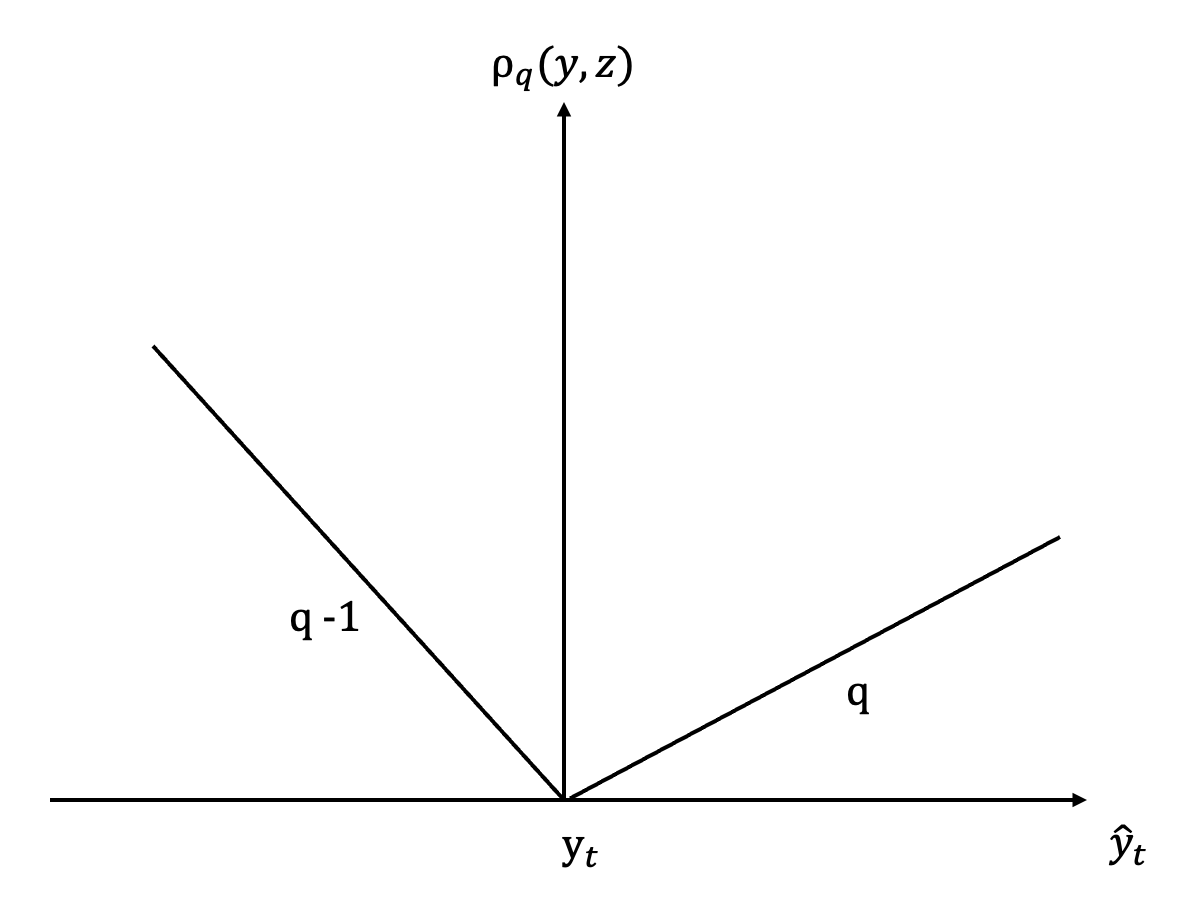
\includegraphics[height=0.5\textheight]{../thesis/images/pinball_loss.png}
    \end{center}
\end{frame}





\begin{frame}{Continous ranked probability score}
The continous ranked probability score (CRPS) measures the difference between the estimated cumulative distribution $\hat{F}$ and the empirical cumulative density function (CDF).
\begin{definition}\label{def_crps}
    The continous ranked probability score is defined as
    $$
    \mathrm{CRPS}(y, \hat{F})=\int\limits_{-\infty}^{\infty}\left(\hat{F}(x)-\mathbb{I}_{\{x-y\}} \right)^2 dx
    $$
\end{definition}
% Nevertheless, we can evaluate the integral in closed form. 
Where the indicator function is defined as 
    $$\mathbb{I}_{\{z\}}=
\begin{cases}
0, & z<0\\
1, & z \geq 0
\end{cases}$$
\end{frame}


\begin{frame}{Continous ranked probability score}
    For a visualisation see Figure. The grey area is what contributes toward the CRPS score.
    The better the estimated cumulative density function is the smaller the total CRPS score will be.
    \begin{figure}
        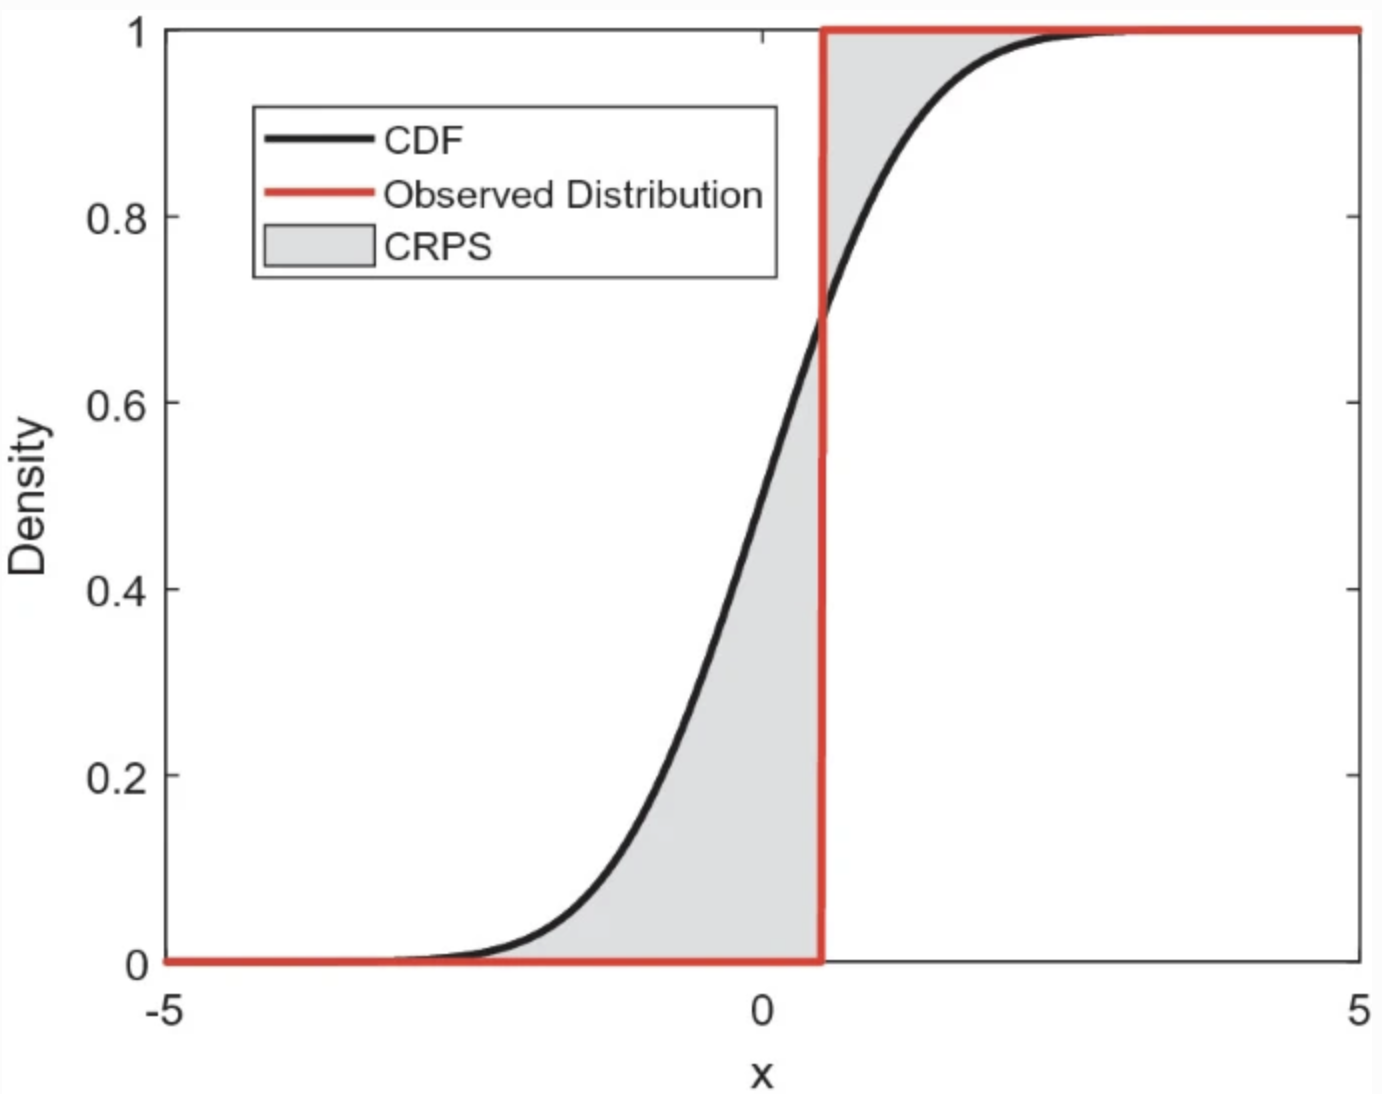
\includegraphics[width=0.5\textwidth]{../thesis/images/crps.png}
    \end{figure}
\end{frame}

% kernel methods
% ch 3
% kernel methods
% ch 3

\section{Kernel theory}

\begin{frame}


\end{frame}

% experiments
% ch 8, 9, 10
Analysis of experiments and results
\\
Building on the theory introduced in \ref{ch:point} and \ref{ch:prob}, this section covers the experiments carried out and the results obtained.

- Comments
\\
- Comparison
\\
- Table of loss scores
\\
Plots:
\\
- Plots for visualizing timeseries with quantiles bounds
\\
- Other plots that will come up to mind

\section{Quantile forecasting}
In this subsection we compare performance of quantile regressor considering the GEFCom2014 dataset.
\\
- experiment for quantile estimator on gefcom2014 and we are good


% results


\begin{frame}{Results}
    \begin{itemize}
        \item We have studied kernel methods for electricity forecasting both in the point and probabilistic framework.
        \item We provided a Python open source implementation for kernel quantile regression compatible with the sklearn API. The code has been packaged and uploaded to the Python Package Index (PyPI) with the name \href{https://pypi.org/project/kernel-quantile-regression/\#2}{kernel-quantile-regression}. The \href{https://github.com/luca-pernigo/kernel_quantile_regression}{github repo} hosting the source code includes also the script implementing the experiments along with the cleaned datasets; this contribution is intended to forster reproducibility in research.
        \item We achieved superior performance of kernel quantile regression compared to standard quantile regressor algorithms. 
        \item We created and made available datasets suitable for algorithms benchmarking considering data from the DACH region (Germany, Switzerland and Austria). The format of these data takes inspiration from the popular GEFCom competitions.
        \item Kernel quantile regression extensive comparison between kernel function types.
        \item We compared kernel quantile regression against state of the art probabilistic algorithms in the literature by means of the GEFCom2014 competition.
    \end{itemize}
\end{frame}

% thank you
\section*{Acknowledgement}  
\begin{frame}

\textcolor{myNewColorA}{\huge{\centerline{Thank you}}}
\vspace*{0.5cm}

%\textcolor{myNewColorA}{\Large{\centerline{E-mail: }}}

\end{frame}



\end{document}




